\subsection{Opgave 35}

Figuren viser grafen for en eksponentialfunktion f.

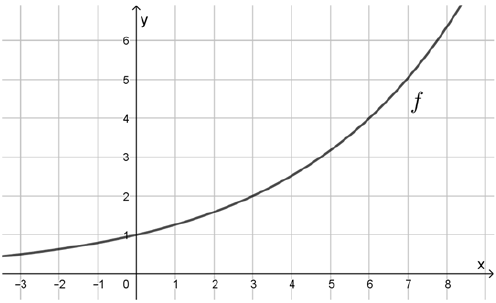
\includegraphics[width=8cm]{Opgave_31-40/Opgave_35/35.png}

Benyt figuren til at bestemme eksponentialfunktionens fordoblingskonstant.

\ans 

For at finde fordoblingskonstanten ud fra en graf skal vi gøre følgende.

Først vælger vi en værdi på y aksen. Jeg vælger $y  = 1$. S
Så går vi ud fra y aksen hvor $y = 1$ indtil vi rammer funktionen f, og aflæser den tilhørende x værdi.
Denne x værdi kalder vi for $x_1$ og aflæser værdien til $x_1 = 1$.

Nu fordobler vi den y værdi vi valgte til at starte med, og får den nye y værdi $y = 2$.
Vi går ud fra y aksen indtil vi rammer funktionen og aflæser den tilhørende x værdi.
Denne x værdi kalder vi for $x_2$ og aflæser værdien til $x_2 = 3$.

Nu kan vi beregne fordoblingskonstanten $T_2$ ved brug af formlen

\begin{align*}
    T_2 = x_2 - x_1
\end{align*}

Indsætter vi værdierne får vi

\begin{align*}
    T_2 = 3 - 1 = 2
\end{align*}

Fordoblingskonstanten for eksponentialfunktionen f er dermed 2.
På nedenstående figur kan man se hvordan de forskellige værdier er blevet aflæst.

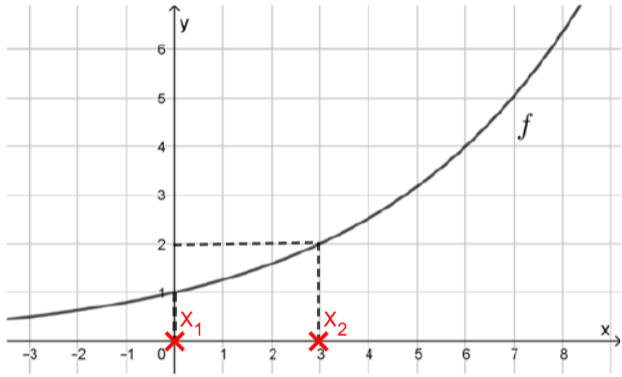
\includegraphics[width=8cm]{Opgave_31-40/Opgave_35/35.1.png}